% -*- coding: utf-8 -*-
%%%%%%%%%%%%%%%%%%%%%%%%%%%%%%%%%%%%%%%%%%%%%%%%%
%%% CHAPTER: Blind Search
%%%%%%%%%%%%%%%%%%%%%%%%%%%%%%%%%%%%%%%%%%%%%%%%%
\chapter{情報なし探索 (Blind Search)}
\label{ch:blind-search}

\ref{ch:introduction}章では様々な状態空間問題を紹介したが、それぞれの問題の解法はどれも沢山研究されている。
一つの指針としては、ある問題に特化した解法を研究することでその問題をより高速に解くというモチベーションがある。
これは例えばMSAのように重要なアプリケーションがある問題の場合に特に熱心に研究されることが多い。
一方、なるべく広い範囲の問題に対して適用可能な手法を研究するというモチベーションもある。
{\bf この章で紹介する手法は問題特化のアルゴリズムよりもパフォーマンスに劣るが、問題の知識をあまり必要とせず、さまざまな問題に適用できる}。
%ただしこのような手法はドメインに特化したプログラムと比べてパフォーマンスに劣ることが多い。

\ref{ch:introduction}章で紹介した状態空間問題を広く扱うことの出来る手法としてグラフ探索アルゴリズムがある。
本章では最もシンプルな問題(ドメイン)の知識を利用しない探索を紹介する。
情報なし探索 (Blind Search)は状態空間グラフのみに注目し、背景にある問題に関する知識を一切使わないアルゴリズムである。
このような探索では{\bf 1. 重複検知を行うか 2. ノードの展開順序}が重要になる。
重複検出は訪問済みの状態を保存しておくことで同じ状態を繰り返し探索することを防ぐ手法である。対価としては、メモリの消費量が非常に大きくなることにある。
ノードの展開順序とは、例えば幅優先探索・深さ優先探索などのバリエーションを指す。
効率的な展開順序は問題によって大きく異なり、問題を選べばこれらの手法によって十分に効率的な探索を行うことが出来る。
これらの探索手法は競技プログラミングでもよく解法として使われる\cite{skiena2006programming}。また、いわゆるコーディング面接でもグラフ探索アルゴリズムは頻出である\cite{mcdowell2011cracking}。
%\ref{ch:search-performance}章はグラフ探索の高速化の紹介をするので、特に競技プログラミングに興味がある場合はそちらも参照されたい。% TODO
情報なし探索は\cite{cormen01}の22章Elementary Graph Algorithmsにも詳しく説明されている。


\section{木探索アルゴリズム (Tree Search Algorithm)}
\label{sec:tree-search-algorithm}
木探索アルゴリズムはグラフ探索アルゴリズムの基礎となるフレームワークであり、本文で紹介する手法のほとんどがこのフレームワークを基礎としているといえる。
アルゴリズム\ref{alg:implicit-tree-search}は木探索の疑似コードである。

\begin{algorithm}[h]
\caption{木探索 (Implicit Tree Search)}
\label{alg:implicit-tree-search}
	\Input{非明示的状態空間グラフ $(s, Goal, Expand, w)$, プライオリティ関数 $f$}
	\Output{$s$からゴール状態への経路、経路が存在しなければ$\emptyset$}
	$Open \leftarrow \{s\}$, $d(s) \leftarrow 0$, $g(s) \leftarrow 0$\;
	\While{$Open \neq \emptyset$} {
                $u \leftarrow \argmin_{u' \in Open} f(u')$ \;
		$Open \leftarrow Open \setminus \{u\} $\;
		\If {$Goal(u)$} {
			\Return $Path(u)$\;
		}
		\For {each $v \in Expand(u)$} {
 			$Open \leftarrow Open \cup \{u\}$\;
		        $d(v) \leftarrow d(u) + 1$\;
		        $g(v) \leftarrow g(u) + w(u, v)$\;
			$parent(v) \leftarrow u$\;
		}
 	}
	\Return $\emptyset$\;
\end{algorithm}
    
木探索はオープンリスト\footnote{歴史的な経緯でリストと呼ばれているが、データ構造がリストで実装されるという意味ではない。効率的なデータ構造は\ref{ch:search-performance}章で紹介する。}と呼ばれるノードの集合をPriority queueに保持する。探索の開始時には、初期状態のみがオープンリストに入っている。
木探索は、このオープンリストから一つノード$u$を選び、ゴール条件を満たしているかを確認する。満たしていれば初期状態から$u$への経路を返す。満たしていなければ、そのノードを展開する。展開とは、そのノードの子ノードを列挙し、オープンリストに入れることを指す。

\begin{figure}
  \centering
  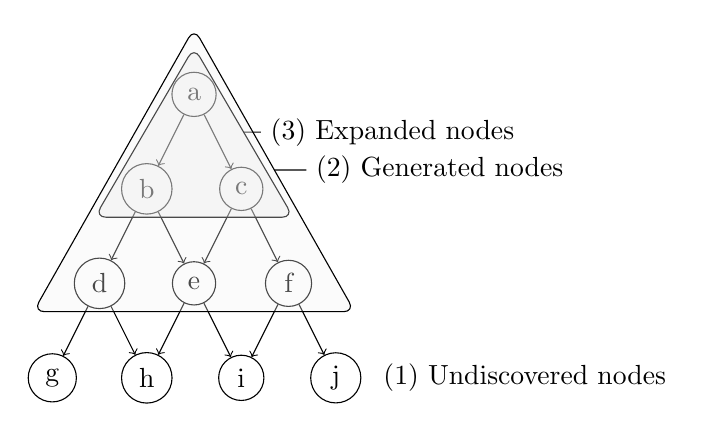
\begin{tikzpicture}[scale=0.6]
    % Reexpansion

\node [draw,circle] (a) at ( 0, 4) {a};

\node [draw,circle] (b) at (-1, 2) {b};
\node [draw,circle] (c) at ( 1, 2) {c};

\node [draw,circle] (d) at (-2, 0) {d};
\node [draw,circle] (e) at ( 0, 0) {e};
\node [draw,circle] (f) at ( 2, 0) {f};

\node [draw,circle] (g) at (-3,-2) {g};
\node [draw,circle] (h) at (-1,-2) {h};
\node [draw,circle] (i) at ( 1,-2) {i};
\node [draw,circle] (j) at ( 3,-2) {j};

\draw[->] (a) -- (b);
\draw[->] (a) -- (c);

\draw[->] (b) -- (d);
\draw[->] (b) -- (e);
\draw[->] (c) -- (e);
\draw[->] (c) -- (f);

\draw[->] (d) -- (g);
\draw[->] (d) -- (h);
\draw[->] (e) -- (h);
\draw[->] (e) -- (i);
\draw[->] (f) -- (i);
\draw[->] (f) -- (j);



% expanded nodes
\draw[rounded corners, fill=gray!20, fill opacity=0.3] (0, 4 + 1) -- (-1 - 1.1, 2 - 0.6) -- (1 + 1.1, 2 - 0.6) -- cycle;

\node (label3) at (4.2, {((4+1) + (2 - 0.6)) / 2}) {(3) Expanded nodes};

\coordinate (draw3) at ({(0 + (1 + 1.1)) / 2}, {((4+1) + (2 - 0.6)) / 2});
\draw[-] (draw3) -- (label3);

% generated nodes
\draw[rounded corners, fill=gray!10, fill opacity=0.3] (0, 4 + 1 + 0.4) -- (-2 - 1.4, 0 - 0.6) -- (2 + 1.4, 0 - 0.6) -- cycle;

\node (label2) at (5.2, {((4+1+0.4) + (0 - 0.6)) / 2}) {(2) Generated nodes};

\coordinate (draw2) at ({(0 + (2 + 1.4)) / 2}, {((4+1+0.4) + (0 - 0.6)) / 2});
\draw[-] (draw2) -- (label2);


\node at (7, -2) {(1) Undiscovered nodes};


  \end{tikzpicture}
  \caption{未生成・生成済み・展開済みノードの例。木探索は生成済みノードのうち展開済みでないものをひとつ取り出し、そのノードを展開し子ノードを得る。新しく得られた子ノードは未生成ノードから生成済みノードとなり、展開したノードは展開済みノードになる。}
  \label{fig:node-life}
\end{figure}

各ノードの注目すると、ノードは1. 未生成、2. 生成済み、3. 展開済みと状態が遷移していく。

\begin{enumerate}
\item 未生成ノード (Undiscovered nodes): 状態空間内のまだ生成されていないノード。非明示的グラフでは情報は保持されていない。
\item 生成済みノード (Generated nodes): オープンリストに一度でも入れられたノード。後述するグラフ探索ではクローズドリストに入れられる。
\item 展開済みノード (Expanded nodes): $Expand$を実行し終えたノード。子ノードがすべて生成済みノードになる。オープンリストからは取り除かれる。
\end{enumerate}

図\ref{fig:node-life}は探索アルゴリズムが$\{a, b, c\}$を展開し終えた時点でのノードの分類の例である。
$\{a, b, c\}$は展開済みノードであり、同時に生成済みノードである。これらのノードは後述するグラフ探索ではクローズドリストと呼ばれるデータ構造に入れられ、保持される。これらのノードの子ノードがすべて生成される。$\{d, e, f\}$は生成済みノードであるが展開済みではない。探索アルゴリズムのオープンリストにはこれらのノードが入っている。$\{g, h, i, j\}$は未生成のノードであり、アルゴリズムからは見えない未発見のノードである。
例えば次に$d$を展開すると、展開済みノードは$\{a, b, c, d\}$となり、新たに$\{g, h\}$が未生成ノードから生成済みノードに遷移する。このように探索が進行していくことによってノードは順次状態遷移していく。


初期状態からノード$n$への最小ステップ数を深さ$d$と呼び、最小経路コストを$g$値と呼ぶ。すべてのアクションのコストが1のドメインであれば任意の$n$に対して$d(n) = g(n)$が成り立つ。
状態を更新すると同時に$g$値を更新する。これによって解を発見した時に解ノードの$g$値が解のコストとなる。
なお、状態$s$に対して適用可能なアクションの集合$A(s)$は与えられていると仮定する。

$Path(u)$はノードに対して初期状態からそこへ到達するまでの経路を返す関数である。$(u, parent(u), parent(parent(u)),...,s)$のように再帰的に$parent$を初期状態まで辿る。

{\bf 紛らわしいが、木探索アルゴリズムは木だけでなくグラフ一般を探索するアルゴリズムである。}
木探索の強みは生成済みノードのうち展開済みではないもののみをオープンリストに保持すればよいことにある。未生成ノード、展開済みノードはメモリ上に保持する必要がない。
一方これの問題は、一度展開したノードが再びExpandによって現れた場合\define{再展開}{reexpansion}{さいてんかい}をすることになる。図\ref{fig:reexpansion}の例ではノード$d$に二通りの経路で到達できるが、木探索では二回目に$d$に到達したとき、すでに到達済みであることを把握できない。そのため同じノードを再び生成・展開することになる。
このように木探索は複数の経路で到達可能なノードがあるほど(グラフがより木から遠いほど)同じノードを何度も再展開することになり、効率が悪くなってしまう。

また、木探索アルゴリズムは状態数が有限であっても停止しない場合がある。
これらが問題になるような問題ドメインである場合は後述する重複検出を使うグラフ探索 (\ref{sec:graph-search-algorithm}節)を使うと良いだろう。


\begin{figure}
  \centering
  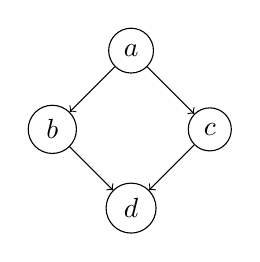
\begin{tikzpicture}[scale=0.5]
    % Reexpansion

\node [draw,circle] (a) at ( 0, 4) {$a$};
\node [draw,circle] (b) at (-2, 2) {$b$};
\node [draw,circle] (c) at ( 2, 2) {$c$};
\node [draw,circle] (d) at ( 0, 0) {$d$};

\draw[->] (a) -- (b);
\draw[->] (b) -- (d);

\draw[->] (a) -- (c);
\draw[->] (c) -- (d);

  \end{tikzpicture}
  \caption{ノードの再展開の例}
  \label{fig:reexpansion}
\end{figure}


オープンリストはプライオリティキューであり、どの順番でノードを取り出すかを決めなければならない。プライオリティ$f$の選択は探索アルゴリズムの性能に強く関係する。
本章の\ref{sec:breadth-first-search}節以降、及び\ref{ch:heuristic-search}章はこのプライオリティをどうデザインするかについて議論をする。

%木探索ベースのアルゴリズムの問題は、解が存在しない場合に停止性を満たさないことである。よって、この手法は解が間違いなく存在することが分かっている問題に対して適用される。あるいは、解が存在することを判定してから用いる。


\section{グラフ探索アルゴリズム (Graph Search Algorithm)}
\label{sec:graph-search-algorithm}


明示的グラフのあるノードが初期状態から複数の経路でたどり着ける場合、同じ状態を表すノードが木探索による非明示的グラフに複数現れるということが生じる。このようなノードを\define{重複}{duplicate}{ちょうふく}と呼ぶ。ノードの重複は計算資源を消費してしまうので、効率的な\define{重複検出}{duplicate detection}{ちょうふくけんしゅつ}の方法は重要な研究分野である。
{\bf 本書ではノードの重複検出を行う探索アルゴリズムを狭義にグラフ探索アルゴリズムと呼び、重複検出を行わない探索を狭義に木探索アルゴリズムと呼ぶ。}


\begin{algorithm}[tbh]
\caption{グラフ探索 (Implicit Graph Search)}
\label{alg:implicit-graph-search}
	\Input{非明示的状態空間グラフ $(s, Goal, Expand, w)$、プライオリティ関数 $f$}
	\Output{$s$からゴール状態への経路、経路が存在しなければ$\emptyset$}
	$Open \leftarrow \{s\}$, $Closed \leftarrow \{s\}$, $d(s) \leftarrow 0$, $g(s) \leftarrow 0$\;
	\While{$Open \neq \emptyset$} {
                $u \leftarrow \argmin_{u' \in Open} f(u')$ \;
		$Open \leftarrow Open \setminus \{u\} $\;
		\If {$Goal(u)$} {
			\Return $Path(u)$\;
		}
		\For {each $v \in Expand(u)$} {
		  \If{$v \notin Closed$ {\bf or} $g(u) + w(u, v) < g(v)$} {
                    $Open \leftarrow Open \cup \{v\}$\;
		    $d(v) \leftarrow d(u) + 1$\;
		    $g(v) \leftarrow g(u) + w(u, v)$\;
                    $parent(v) \leftarrow u$\;
                  }
		  \If{$v \notin Closed$} {
                    $Closed \leftarrow Closed \cup \{v\}$\;
                  }
		}
 	}
	\Return $\emptyset$\;
\end{algorithm}


重複検出のためには生成されたノードを\define{クローズドリスト}{closed list}{クローズドリスト}に保存する。一度クローズドリストに入れられたノードはずっとクローズドリストに保持される。
ノード展開関数から子ノードが生成されたら、その子ノードと同じ状態を保持するノードがクローズドリストに存在するかを確認する。
もし存在しなければ、そのノードは重複ではない。なのでそのノードをオープンリストに加える。
存在した場合の処理は少しややこしい。
新たに生成されたノード$n$の$g$値のほうが先に生成されクローズドリストにあるノード$n'$の$g$値よりも小さい場合が存在する。このとき、$n$をそのまま捨ててしまうと、そのノードの$g$値が本来の値よりも大きく評価されてしまう。

$g$値をそのノードに到達できる既知の最小コストにするためには、まずクローズドリストに保存されているノードの$g$値を$g(n')$から$g(n)$に更新しなければならない。
加えて、ノード$n$を\define{再展開}{reexpansion}{さいてんかい}しなければならない。
ノード$n$の子ノード$c$は$n'$の子ノードとして展開されていたわけであるが、そのとき$g(c) = g(n') + w(n', c)$として計算された。この値は$g(c) = g(n) + w(n, c)$に更新しなければならない。$w(n', c) = w(n, c)$なので、$g(n') - g(n)$だけ$g$値が小さくなる。なので、$c$の子ノードも再展開をする必要がある。そしてそのまた子ノードも。。。というように、再展開が生じるとそこから先のノードをすべて再展開する必要がある。これはかなり大きなコストになることが多いので、可能な限り避けたい処理である。

%なので常に$g$値をそのノードに到達できる既知の最小コストに更新する。

重複が存在した場合に必ずノードを捨てることができる場合も存在する。
まず、解の最適性が必要でない場合$g$値を更新する必要はない。$g$値が過大に評価されても解経路は解経路のままであり、ただ解経路のコストが大きくなるだけである。
また、例えば幅優先探索では探索の過程で生成されるノードの$d$値は単調増加する。もしユニットコストドメインならば$g$値も単調増加である。つまりノード$n$と重複したノード$n'$がクローズドリストにあったとすると、$g(n) \geq g(n')$が成立する。この場合、解最適性を保ったまま$n$を安全に捨てることができる。
また、状態空間グラフが木である場合は重複が発生しない。
なお、後述するA*探索\ref{sec:astar-search}ではある条件を満たせば再展開は行わずに解の最適性が満たせることが知られている。これがA*探索がstate-of-the-artとして重要視されている理由である。

ここで「ノード」と「状態」の言葉の使い分けに注意したい。
状態とは状態空間問題における状態$s$である。ノードは状態$s$を含み、$f$値、$g$値の情報を含む。
重複検出を行わない木探索の場合、同じ状態を保持するノードが2つ以上存在しうる。
重複検知は同じ状態を保持するノードをマージする処理に相当する。この処理を行うと同じノードに複数の経路で到達するようになり、グラフは木ではなくなる。

% 重複検出を行ってもノードの再展開が必要になる場合は存在するが、ほとんどの場合重複検出を行わない場合よりもはるかに再展開の回数は少なくなる。
% 実行時間で見ると重複検出を行ったほうがほぼ確実に効率的である。
重複検出の問題はメモリの使用量である。重複検出を行うためには生成済みノードをすべてクローズドリストに保存しなければならない。なので展開済みノードの数に比例した空間が必要になる。
クローズドリストの効率的な実装については\ref{sec:closed-list}節で議論をする。

なお、重複検出はノードが生成されたときではなく、ノードが展開されるときに遅らせることができる。
オープンリストには重複したノードが含まれることになるが、ノードの展開時には重複をチェックするので重複したノードの展開は防げる、ということである。これは\define{遅延重複検出}{delayed duplicate detection}{ちえんちょうふくけんしゅつ}と呼ばれ、\ref{sec:delayed-duplicate-detection}節で議論をする。



\section{幅優先探索 (Breadth-First Search)}
\label{sec:breadth-first-search}

探索のパフォーマンスにおいて重要になるのは{\bf どのようにして次に展開するノードを選択するか}にある。
ヒューリスティック探索の研究の非常に大きな部分はここに費やされているといえる。
シンプルかつ強力なノード選択方法はFirst-in-first-out (FIFO)である。あるいは幅優先探索と呼ぶ。

幅優先探索の手順は非常に単純であり、FIFOの順に$Open$から取り出せばいいだけである。
これをもう少し大きな視点で、{\it どのようなノードを優先して探索しているのか}を考えてみたい。
初期状態から現在状態にたどり着くまでの経路の長さをノードの$d$値と定義する。
すると、幅優先探索のプライオリティ関数$f$は$d$値と一致する。

\begin{equation}
  f_{\text{brfs}}(s) = d(s)
\label{alg:brfs-open}
\end{equation}

ユニットコスト問題である場合、更に$g$値とも一致する ($f_{\text{brfs}}(s) = d(s) = g(s)$)。

幅優先探索のメリットは最初に発見した解が最短経路長の解であることである。
問題がユニットコストドメインであれば、最短経路が最小コスト経路であるので、最適解が得られる。
なお、後述するBest First Searchと区別するため、Breadth-First Searchの略称はBrFSを用いることがある (Best First SearchはBFSとなる)。

重複検出を用いた幅優先探索で図\ref{fig:ssp-graph}の問題を解こうとすると、オープンリスト、クローズドリストの中身は表\ref{tbl:brfs-traj}のように遷移する。
図\ref{fig:ssp-tree}の探索木を見比べながら確認してみてほしい。

\begin{figure}
  \centering
  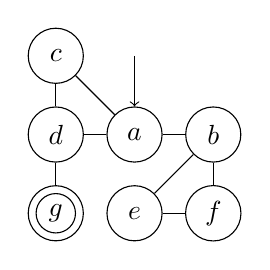
\begin{tikzpicture}[scale=0.5]
    % MDP i
\node [draw, circle, minimum size=0.7cm] (a) at (2, 2) {$a$};
\node [draw, circle, minimum size=0.7cm] (b) at (4, 2) {$b$};
\node [draw, circle, minimum size=0.7cm] (c) at (0, 4) {$c$};
\node [draw, circle, minimum size=0.7cm] (d) at (0, 2) {$d$};
\node [draw, circle, minimum size=0.7cm] (e) at (2, 0) {$e$};
\node [draw, circle, minimum size=0.7cm] (f) at (4, 0) {$f$};
\node [draw, circle, minimum size=0.7cm] (g) at (0, 0) {$g$};
\node [draw, circle, minimum size=0.5cm] at (0, 0) {};

\coordinate[above of=a] (init);

\draw[->] (init) -- (a);
\draw[-] (a) -- (b);
\draw[-] (a) -- (c);
\draw[-] (a) -- (d);
\draw[-] (b) -- (e);
\draw[-] (b) -- (f);
\draw[-] (c) -- (d);
\draw[-] (d) -- (g);
\draw[-] (e) -- (f);
\draw[-] (d) -- (g);

  \end{tikzpicture} \hspace{20pt}
  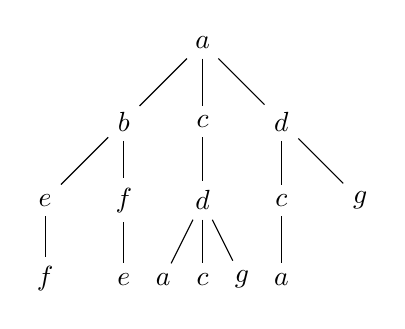
\begin{tikzpicture}[scale=0.5]
    % MDP i
\node (a0) at (4, 6) {$a$};

\node (b1) at (2, 4) {$b$};
\node (c1) at (4, 4) {$c$};
\node (d1) at (6, 4) {$d$};

\node (e2) at (0, 2) {$e$};
\node (f2) at (2, 2) {$f$};
\node (d2) at (4, 2) {$d$};
\node (c2) at (6, 2) {$c$};
\node (g2) at (8, 2) {$g$};

\node (f3) at (0, 0) {$f$};
\node (e3) at (2, 0) {$e$};
\node (a31) at (3, 0) {$a$};
\node (c3) at (4, 0) {$c$};
\node (g3) at (5, 0) {$g$};
\node (a32) at (6, 0) {$a$};

\draw[-] (a0) -- (b1);
\draw[-] (a0) -- (c1);
\draw[-] (a0) -- (d1);
\draw[-] (b1) -- (e2);
\draw[-] (b1) -- (f2);
\draw[-] (c1) -- (d2);
\draw[-] (d1) -- (g2);
\draw[-] (d1) -- (c2);
\draw[-] (e2) -- (f3);
\draw[-] (f2) -- (e3);
\draw[-] (d2) -- (a31);
\draw[-] (d2) -- (c3);
\draw[-] (d2) -- (g3);
\draw[-] (c2) -- (a32);

  \end{tikzpicture}
  \caption{探索木}
  \label{fig:ssp-tree}
\end{figure}


\begin{table}[tbh]
\centering
\caption{重複検出を用いた幅優先グラフ探索のオープンリスト・クローズドリスト (\cite{edelkamp:2010:hst:1875144}より)}
\begin{tabular}{c|c|l|l|l}
  \toprule
	ステップ & ノードの選択 & オープンリスト & クローズドリスト & コメント \\ \midrule
	1 	  & \{\}       & \{a\}      & \{\} \\
	2     & a        & \{b,c,d\}  & \{a\} \\
	3     & b        & \{c,d,e,f\} & \{a,b\} \\
	4     & c        & \{d,e,f\}   & \{a,b,c\} \\
	5     & d        & \{e,f,g\}   & \{a,b,c,d\} \\
	6     & e        & \{f,g\}     & \{a,b,c,d,e\} \\
	7     & f        & \{g\}       & \{a,b,c,d,e,f\} \\
	8     & g        & \{\}        & \{a,b,c,d,e,f,g\} & ゴール \\
        \bottomrule
\end{tabular}
\label{tbl:brfs-traj}
\end{table}

\section{深さ優先探索 (Depth-First Search)}
\label{sec:depth-first-search}

幅優先探索が幅を優先するのに対して深さ優先探索はもっとも深いノードを優先して探索する。

\begin{equation}
  f_{\text{dfs}}(s) = -d(s)
\label{alg:dfs-open}
\end{equation}

深さ優先探索は解がある一定の深さにあることが既知である場合に有効である。
例えばTSPは全ての街を回ったときのみが解であるので、街の数が$n$であれば全ての解の経路長が$n$である。
このような問題を幅優先探索で解こうとすると、解は最も深いところにしかないので、最後の最後まで解が一つも得られないということになる。一方、深さ優先探索なら$n$回目の展開で一つ目の解を見つけることが出来る。
表\ref{tbl:dfs-traj}は図\ref{fig:ssp-graph}の問題で重複検出ありの深さ優先探索を行った場合のオープンリスト・クローズドリストの遷移を示した。図\ref{fig:ssp-tree}と合わせてノードが展開される順序を確認すると良い。

深さ優先探索は無限グラフにおいて、解が存在しても永遠に停止しない場合がある。幅優先探索であれば解がある場合、いずれそれを発見する (解の深さを$d^*$とすると、$d(s) \leq d^*$であるノードの数は有限であるので)。しかし深さ優先探索は停止しない場合がある。

良い解、最適解を見つけたい場合でも深さ優先探索が有用である場合がある。
早めに一つ解が見つけられると、その解よりも質が悪い解にしかつながらないノードを\define{枝刈り}{pruning}{えだがり}することが出来る。ノード$n$を枝刈りするとは、ノード$n$をオープンリストに加えずそのまま捨てることを指す。つまりアルゴリズム\ref{alg:implicit-tree-search}における$Open \leftarrow Open \cup \{v\}$をスキップする。このような枝刈りを用いた探索アルゴリズムを\define{分枝限定法}{Branch-and-Bound}{ぶんしげんていほう}と呼ぶ。

\begin{table}[tbh]
\centering
\caption{重複検出を用いた深さ優先グラフ探索のオープンリスト・クローズドリスト (\cite{edelkamp:2010:hst:1875144}より)}
\begin{tabular}{c|c|l|l|l}
  \toprule
	ステップ & ノードの選択 & オープンリスト   & クローズドリスト & コメント \\ \midrule
	1 	  & \{\}     & \{a\}       & \{\} \\
	2     & a        & \{b,c,d\}   & \{a\} \\
	3     & b        & \{e,f,c,d\} & \{a,b\} \\
	4     & e        & \{f,c,d\}   & \{a,b,e\} \\
	5     & f        & \{c,d\}     & \{a,b,e,f\} \\
	6     & c        & \{d\}       & \{a,b,e,f,c\} \\
	7     & d        & \{g\}       & \{a,b,e,f,c,d\} \\
	8     & g        & \{\}        & \{a,b,e,f,c,d,g\} & ゴール \\
        \bottomrule
\end{tabular}
\label{tbl:dfs-traj}
\end{table}

\subsection{再帰による深さ優先探索}
\label{sec:recursive-depth-first-search}

上述の実装はオープンリストを利用した深さ優先探索である。
アルゴリズム \ref{alg:implicit-tree-search}を元にした深さ優先探索の実装は効率的ではないことが多い。
深さ優先探索は再帰によって効率的に実装することができる (アルゴリズム \ref{alg:recursive-dfs})。
再帰実装ではオープンリストがないことに注目したい。
再帰を利用することでデータ構造を明に保存する必要がなくなり、キャッシュ効率が良くなることがある。
幅優先探索も同様に再帰によって実装することが出来るが、効率的であるケースはあまりない。

\begin{algorithm}[tbh]
\caption{DFS: 再帰による深さ優先探索 (Depth-First Search)}
\label{alg:recursive-dfs}
	\Input{非明示的状態空間グラフ $(s, Goal, Expand, w)$、前状態 $s'$}
	\Output{$s$からゴール状態への経路、経路が存在しなければ$\emptyset$}
	\If {$Goal(s)$} {
		\Return $s$\;
	}
	\For {each $u \in Expand(s) \setminus \{s'\}$} {
          $v \leftarrow DFS(u, Goal, Expand, w, s)$\;
	  \If {$v \neq \emptyset$} {
	    \Return $(s, DFS(v, Goal, Expand, w, u))$
	  }
	}
	\Return $\emptyset$\;
\end{algorithm}


\section{ダイクストラ法 (Dijkstra Algorithm)}
\label{sec:dijkstra}

\define{ダイクストラ法}{Dijkstra's Algorithm}{ダイクストラほう}はグラフ探索アルゴリズムの一種であり、グラフ理論の教科書な
どでも登場する情報科学全体に多岐に渡り重要とされるアルゴリズムである \cite{dijkstra1959note}。
例えばネットワークルーティングにおけるlink state algorithmなどにDijkstraが使われる\cite{mcquillan1980new}。
%初期状態からノード$n$への既知の最小経路コストを$g$値と呼び、$g(n)$と書く。
ダイクストラ法はグラフ探索において$g$値が最も小さいノードを優先して展開するアルゴリズムと説明することができる。

\begin{equation}
  f_{\text{bfs}}(s) = g(n)
\end{equation}

{\bf ダイクストラ法は重複検出を行うグラフ探索アルゴリズムである。}
ダイクストラ法は非負コストグラフにおいて最短経路を返す。
ユニットコストドメインでは$\forall n (g(n) = d(n))$であるため、幅優先探索と同じ動作をする。
フィボナッチヒープを用いてオープンリストを実装したダイクストラ法は$O(|E| + |V|log|V|)$時間でであることが知られている\cite{fredman1987fibonacci}。
そのため、後述するヒューリスティック関数が得られない問題においてはとりあえずダイクストラ法を試してみることは有効である。


\section{情報なし探索の比較}
\label{sec:blind-comparison}

探索アルゴリズムの評価指標としては以下の四点が重要である。

\begin{enumerate}
\item 完全性: 解が存在するとき、有限時間内に解を返すか。
\item 最適性: 最初に発見された解が最適解か。
\item 時間: アルゴリズムの実行にかかる時間
\item 空間: アルゴリズムの実行にかかる空間
\end{enumerate}

完全なアルゴリズムであることは有用だが、時間・空間とのトレードオフにあることが多い。
完全であっても実現可能な時間・空間で実行することが出来なければ意味がないので、完全でない高速なアルゴリズムを選択する方が良い場合もある。
最適性も同様に時間・空間とのトレードオフにあることが多いので、解きたい問題に最適な解が必要かどうかを考える必要がある。
また、後述するwA* (節\ref{sec:weighted-astar-search})は発見された解が最適解のコスト$c^*$の定数倍以下であることを保証する近似アルゴリズムである。


表\ref{tbl:comparison}は情報なし探索をこれら四点で比較している。
反復深化深さ優先は節\ref{sec:depth-first-iterative-deepening}、両方向探索は節\ref{sec:bidirectional-search}で紹介する。
$b$は分枝数、$d$は解の深さ、$m$は可能な探索木の深さの最大値である。
重複検出を行うグラフ探索の場合、深さ優先探索は有限グラフならば完全であり、時間・空間は状態空間の大きさ$|S|$でバウンドされる。
この表にある時間・空間量は理論的な最悪の場合の比較である。解きたい問題にかかる平均的な性能は必ずしもこれに相関しない。最終的には実験的なベンチマークを行い良いアルゴリズムを選択する必要がある。

\begin{table}[tbh]
\centering
\caption{木探索アルゴリズムの比較 (\cite{russelln03}のFigure 3.21より)}
\resizebox{\textwidth}{!}{
\begin{tabular}{c|cccc}
  \toprule
  性能  & 幅優先探索 & 深さ優先探索 & 反復深化深さ優先 & 両方向幅優先探索 \\ \midrule
  完全性 & 局所有限グラフならYes & No & 局所有限グラフならYes & 局所有限グラフならYes \\
  最適性 & ユニットコストならYes & No & ユニットコストならYes & ユニットコストならYes \\
  時間  & $O(b^d)$ & $O(b^m)$ & $O(b^d)$ & $O(b^{d/2})$ \\
  空間  & $O(b^d)$ & $O(bm)$  & $O(bd)$ & $O(b^{d/2})$ \\
  \bottomrule
\end{tabular}
}
\label{tbl:comparison}
\end{table}


\section{Python実装}

情報なし探索は様々な言語でライブラリが開発されているため、参考に出来る実装例が多い。
本書では理解の助けとなるために紹介することが目的であるため、既存のライブラリは用いない実装を示す。

Pythonによる木探索は例えば以下のように実装できる。

\inputpython{python/tree_search.py}{1}{74}

\code{TreeSearch}は状態空間問題とプライオリティ関数 \code{priority\_f} を引数に取る。

このコードに重複検出を加えたグラフ探索は以下のように実装できる。

\inputpython{python/graph_search.py}{1}{74}

\code{priority\_f}を適当に渡すことで本章で紹介した幅優先探索、深さ優先探索、ダイクストラ法を実行することができる。

例えば幅優先探索・深さ優先探索は以下のように数行で実装が出来る。

\inputpython{python/breadth_first_search.py}{1}{4}
\inputpython{python/depth_first_search.py}{1}{4}

そして次章で紹介するヒューリスティック探索の手法も実はこの\code{priority\_f}を渡すことで実装ができる。

\section{まとめ}

状態空間問題を解くための手法としてグラフ探索アルゴリズムがある。グラフ探索アルゴリズムは1. 展開するノードの順序と2. 展開したノードの処理の2点で特徴づけることが出来る。
{\it 幅優先探索}は{\it オープンリスト}の中から深さが浅いノードから優先して探索し、{\it 深さ優先探索}は逆に深いノードから優先して探索する。{\it ダイクストラ法}はコストが小さいノードから優先して探索するため、最短経路を最初に見つけることができる。
木探索は展開したノードを保持せず同じ状態を複数回重複して展開してしまうリスクがある。グラフ探索は展開済みノードを{\it クローズドリスト}に保存しておくことで重複展開を防ぐ。一方メモリ消費量が大きくなるというデメリットがある。

探索アルゴリズムの選択において考慮するべきことは主に以下の4点である。解が存在するとき、有限時間内に解を返すか ({\it 完全性})、最初に発見された解が最適解か (最適性)、アルゴリズムの実行にかかる時間と空間。


\section{練習問題}

\begin{enumerate}
	\item 幅優先木探索を実装し、$3 \times 3$のスライディングタイルを解いてみよう。

	\item 重複検出を使った幅優先探索を実装し、$3 \times 3$のスライディングタイルを解いてみよう。重複検出を使わない幅優先木探索と比べて展開したノードの数は?重複検出によって枝刈りされたノードの数は?
	
	\item 重複検出を使った深さ優先探索を実装し、$3 \times 3$のスライディングタイルを解いてみよう。見つけた解は1, 2で見つけた解と比べて長いか?
	
	\item 重複検出を使った幅優先探索で巡回セールスパーソン問題を解いてみよう。この時、見つかった解は最短経路だったか?
	
	\item ダイクストラ法を実装し、巡回セールスパーソン問題を解いてみよう。この時、見つかった解は最短経路だったか?
\end{enumerate}


\section{関連文献}

時間・空間制約が厳しい場合は反復深化探索、両方向探索や並列探索を使えば解決できることがある。
これらのアルゴリズムについては\ref{ch:heuristic-search-variants}章で紹介する。

ダイクストラ法はコストが負のエッジを持つ場合にうまくいかない。
負のエッジを含む問題を解くための手法としてはベルマン-フォード法が有名である \cite{bellman1958routing,ford1956network}。

No Free Lunch定理\cite{wolpert1997no}はコンピュータサイエンスの多くの最適化問題で言及される定理である。
状態空間問題におけるNo Free Lunch定理の主張はざっくりと説明すると以下である。
\dtheorem{
すべての可能なコスト関数による状態空間問題のインスタンスの集合を考える。
この問題集合に対する平均性能はすべての探索アルゴリズムで同じである。
}
つまり、問題の知識が何もなければ「効率的なアルゴリズム」というものは存在しない。
問題に対して知っている知識を利用することによってはじめて探索を効率的にすることができる。
すなわち、状態空間問題のインスタンスの一部分で性能を犠牲にすることで、他のインスタンス集合への性能を向上させることができる。例えば解の長さが20以下であるという知識があるとすれば、探索を深さ20までで打ち切ると良いと考えられる。この探索アルゴリズムは解の長さが20以下であるインスタンスに対しての性能は良くなるが、解の長さが20より大きいインスタンスの性能は著しく悪くなる。このように知識を利用して探索の方向性を変えることがグラフ探索では重要になる。
それが次章で扱うヒューリスティック探索の肝である。


